\chapter{Monte Carlo Computational Techniques}

The name Monte Carlo method is a set of mathematical tools that was first used by scientists working on nuclear projects in Los Alamos. The essence of this is to generate numbers with probability that can be used to study physical phenomena. In our context, the definition of Monte Carlo method is the use of randomly generated numbers to imitate a physical behaviour that is considered to be random (quantum mechanical) \citep{montecarlo}.

%\section{Generating Random Numbers with different PDFs}

One of the most important components of the Monte Carlo method is generating samples of different probability distribution functions (pdf). This is essential since we are simulating various variables that have different numerical behaviour. For example if our pseudo-random numbers are uniformly\footnote{Uniform means that every value in the range of the distribution is equally likely to occur. This distribution is widely used for generating random numbers for other distributions, it is denoted by $U$.} distributed in the interval $[0,1]$  and instead we need numbers that have normal distribution restricted to the same interval. This part of the essay  discusses two methods which are widely used.


\section{The Inverse Transform Method}

The inverse transform method is used for generating random numbers that are distributed according to a specific distribution. 

Let $x$ be a random variable distributed with probability density function $p(x)$. Let $u$ be a random variable that is uniformly distributed in $[0,1]$ and $P(x)$ is the cumulative density function (CDF), then we set 
\begin{equation}
x = P^{-1} (u)
\end{equation}\citep{Weinzierl}.

   
The following pseudo-code shows the inverse-transform method algorithm 
\begin{algorithmic}
\State Generate a uniform  random $u$ in $[0,1]$
\State \Return $x = P^{-1}(u)$
\end{algorithmic}

The inversion method is exact when an explicit form of the CDF is known. The CDF is a continuous and a strictly increasing function. It can be obtained either analytically through the integration of the PDF or numerically. Sometimes finding the CDF if computationally difficult, this causes the inverse transform method to become less efficient \citep{Devroye:1986:SNR:318242.318443}.

\section{The Accept Reject Method}
As the inverse transform method, the accept reject method also is used for generating numbers according to a specific distribution.

Let $x$ be a uniformly distributed variable in the interval $[0,1]$, which is the variable of interest. A different distribution of $x$ is required, let $p(x)$ denotes the pdf of the required distribution. Another  random uniformly distributed variable $y$ is generated, this will serve as the accept reject tool. First we calculate the maximum of $p(x)$, hence the $y$ is generated in the interval $[0,p(x)_{max}]$. Now we check if $y$ $\leq$ $p(x)$. If this is the case, accept $x$, otherwise reject and start again. 
\begin{algorithmic} 
\State $x \gets$ uniform in $[0, 1]$
\State $y \gets$ uniform in $[0, p_{max}(x)]$
\If {$y \leq p(x)$}
    \State accept $x$
\Else 
	\State Reject 
\EndIf
\State Begin again
\end{algorithmic}
%Assume we have access to a sample which is distributed according to the pdf $f(x)$,
%and the let us denote the pdf of the required distribution by $p(x)$, we assume that for both $p(x)$ and $f(x)$ varies over a finite interval.
% 
%In simple words, first we generate $x$ according to the uniform distribution over a given interval assume $[0,1]$ 
%, then we find the maximum of $f(x)$, and then calculates $p(x)$, then we generate another number $y$ which is also uniformly distributed over the interval $[0,f_{max}(x)]$, and checks  $y \times f(x) \leq p(x)$.

%If this the case then accept $x$, if not reject $x$ and start again,
 
For example, if we have a number $x$ that falls under uniform distribution and we want to reshape this so that we get a number  that has the distribution $\frac{1}{x}$, then we find the maximum value of probability density function ($p(x)$) for $x$. Here, we add small number to $x$ so that we avoid the singular point when $x = 0$. After that we generate another sample $y$ that is also uniformly distributed in the interval $[0,p_{max}]$. 
Now we check if $y $ is less than $p(x)$. If so, we add $x$ to our distribution, if not we start again \citep{Weinzierl}. 
%\begin{lstlisting}
%eps = 0.01 #this value to avoid the singular point at x=0 
%while True:
%	x = uniform(0,1) #uniformly distributed in the interval [0,1] 
%	y = uniform(0, 1/eps)#uniformly distributed in the interval[0,f_{max}]
%	if y<=f: #checking the accept reject condition
%		return x
%\end{lstlisting} 

The histogram in figure \ref{fig:2} demonstrate the example above. 
%For the python code see \verb+Accept_reject.py+. 

\begin{figure}[hbtp]
\centering
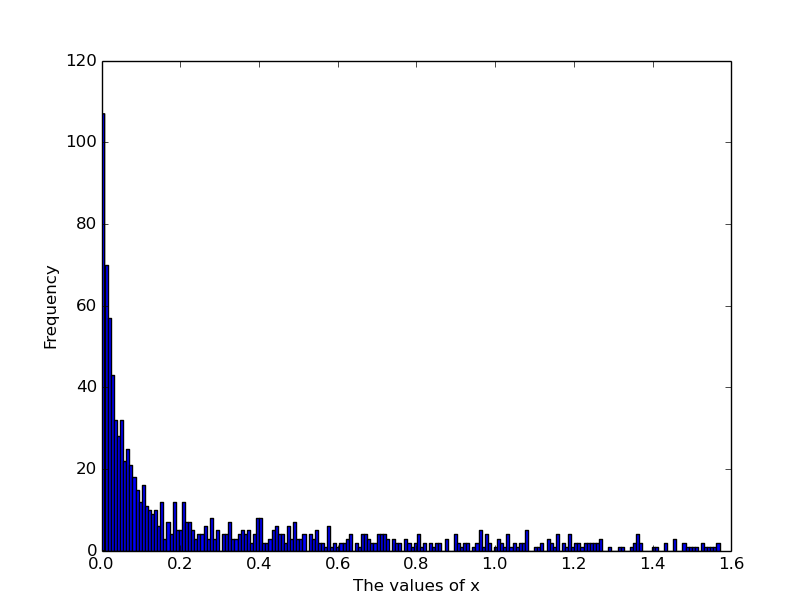
\includegraphics[scale=.5]{images/inverse_method.png}
\caption{Sampling 1000 numbers with distribution $\frac{1}{x+\epsilon}$ using accept-reject method, where $\epsilon$ is a small number added to avoid the singularity.}\label{fig:2}
\end{figure}

Beside the fact that the numbers which are generated from Monte Carlo method  are not truly random, whereby the numbers are generated through a deterministic algorithms  \citep{montecarlo}. Monte Carlo method also faces another challenge which it requires generating large samples to give sensible results. The histograms in figure \ref{fig:1.1} demonstrate that, in which $pi$ is calculated using numbers generated using Monte Carlo method.    
One sees that the error in the calculation when is decreasing as the number of the samples is increasing .

 

%In contrast, the efficiency of accept -reject algorithm does not depend that much on the shape of the pdf.
%Moreover, the accept - reject method does not require the evaluation of the CDF. 

%The following example demonstrate the efficiency of accept - reject method in which the value of $\pi$ is calculated using the accept - reject method.


%Assume we have a box of side length D and a circle of diameter D inside the box, the probability that a point in the box is also in the circle is approximately the area of the circle over the area of the box, that is, $\pi$ over 4. 
%From this we can approximate the value of $\pi$. 
%The histograms in Figure \ref{fig:1.1} exhibits this calculation and also the error in the calculation. 
%For the python code see \verb+Calculation_of_pi.py+ and \verb+uncertainity_in_pi_calculation.py+.

\begin{figure}
    \centering
    \begin{subfigure}[b]{0.5\textwidth}
        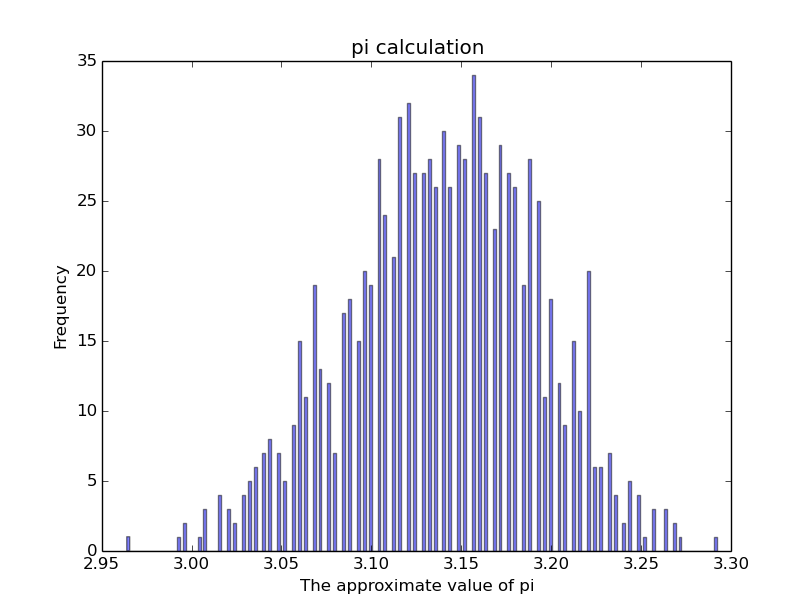
\includegraphics[scale=.5]{images/pi_value.png} 
        \caption{pi value}
        \label{fig:gull}
    \end{subfigure}
    ~ %add desired spacing between images, e. g. ~, \quad, \qquad, \hfill etc. 
      %(or a blank line to force the subfigure onto a new line)
    \begin{subfigure}[b]{0.5\textwidth}
        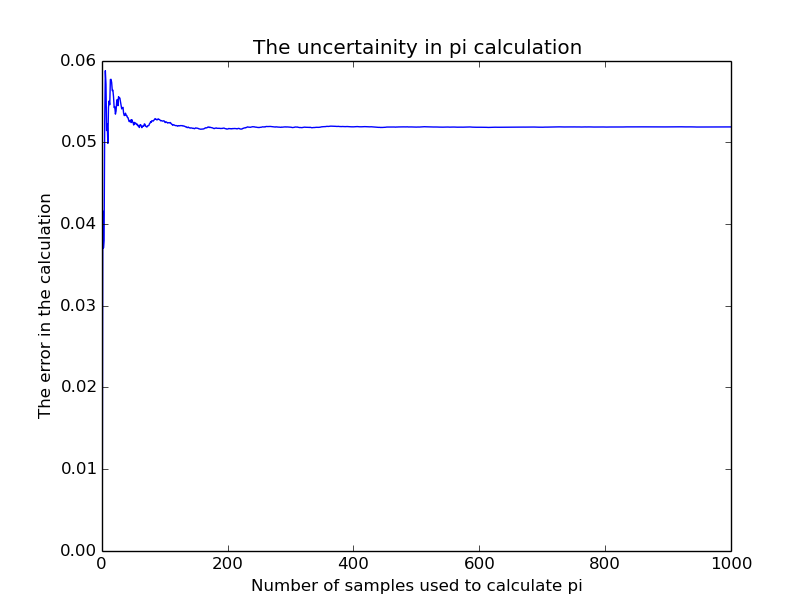
\includegraphics[scale=0.5]{images/uncertainity_pi.png}
        \caption{The uncertainty}
        \label{fig:tiger}
    \end{subfigure}
    \label{Fig:1}
\caption{These histograms show the values of $\pi$ (a) and the error that are generated from sampling 1000 numbers (b).} 
\label{fig:1.1}
\end{figure}           